\chapter{Architectuur}\label{ch:Architectuur}

Om inzicht te verkrijgen in potentiële kwetsbaarheden in de projecten van Eaglescience moet er een applicatie worden ontworpen die analyses kan uitvoeren op het moment dat er veranderingen worden aangebracht in deze projecten. Daarnaast moet de applicatie in staat zijn deze analyses uit te voeren op een periodieke basis.
Op het moment van schrijven wordt er binnen Eaglescience ontwikkeld in de talen Scala en TypeScript, maar de verwachting is dat er in de toekomst een mogelijkheid bestaat dat dit uitgebreid gaat worden. Daarnaast zijn deze twee talen niet de enige twee platformen binnen de stack, maar wordt er ook gebruik gemaakt van docker met daarbij verschillende images die ook kwetsbaarheden kunnen bevatten. Dit ontwerp voorziet niet in de mogelijkheid om deze toekomstige platformen (als Docker) te kunnen scannen, echter zal het wel de mogelijkheid bieden om deze op een relatief makkelijke manier later toe te voegen. De selectie van deze toekomstige tool moet wel de mogelijkheid bieden om te voorzien in de data beschreven in het interne datamodel.

Analyses worden uitgevoerd op module niveau, hier zijn in basis twee redenen voor. Ten eerste is een module binnen een Eaglescience project een afgeschermd onderdeel dat een eigen platform benut. Ten tweede kunnen er op module niveau veranderingen worden verwacht ten opzichte van dependency declaraties.

Als de architectuur wordt gebasseerd op het datamodel kan er vervolgens worden gekeken welke componenten en technieken er nodig zijn om het datamodel functioneeel te krijgen.

\section{Datamodel}\label{sec:datamodel}
Om de gebruiker in staat te stellen om een gedegen keuze te maken om over te gaan op het updaten van de applicatie is een zo actueel mogelijk beeld nodig van de huidige situatie omtrent kwetsbaarheden in een project. Om deze informatie kunnen bieden is er gekozen om dit te bieden op twee niveau's en dus door middel van twee datamodellen.
Het eerste datamodel is onderdeel van de SOUP-API en wordt hieronder verder refereert als het interne datamodel. Daarnaast is er een model dat binnen de Portal gebruikt wordt voor het opslaan van samengevatte gegevens verder benoemd als het Portalmodel.

%TODO: Kijken of er een ranking high ,medium etc aanwezig is. enhoe deze is opgebouwd.
\subsection{Interne datamodel}\label{subsec:interne-datamodel}
Het interne datamodel is opgebouwd op basis van de data die wordt verkregen van de in het onderzoek gevonden OWASP tools. Hieruit kan worden gedestileerd welke gegevens daadwerkelijk nodig zijn voor de functionaliteit die wordt verwacht binnen Eaglescience. Het in figuur~\ref{fig:SOUP-SoupApiDm} getoonde model laat deze destillatie zien. Centraal in het datamodel staat de analyse. De analyse is aan modules gekoppeld omdat de rapportages uit de SCA tooling gebasseerd zijn op modules en niet op projecten. Het project is een verzameling modules dat in zijn geheel een applicatie vormt. De analyse zelf is opgebouwd uit de dependency files, welke opgeslagen worden om in de toekomst periodieke analyses uit te kunnen voeren tot er een nieuwe analyse is. Ook worden alle dependencies opgeslagen waarin gevonden vulnarabilities en bewijs worden opgeslagen.

\begin{figure}[H]
    \myfloatalign
    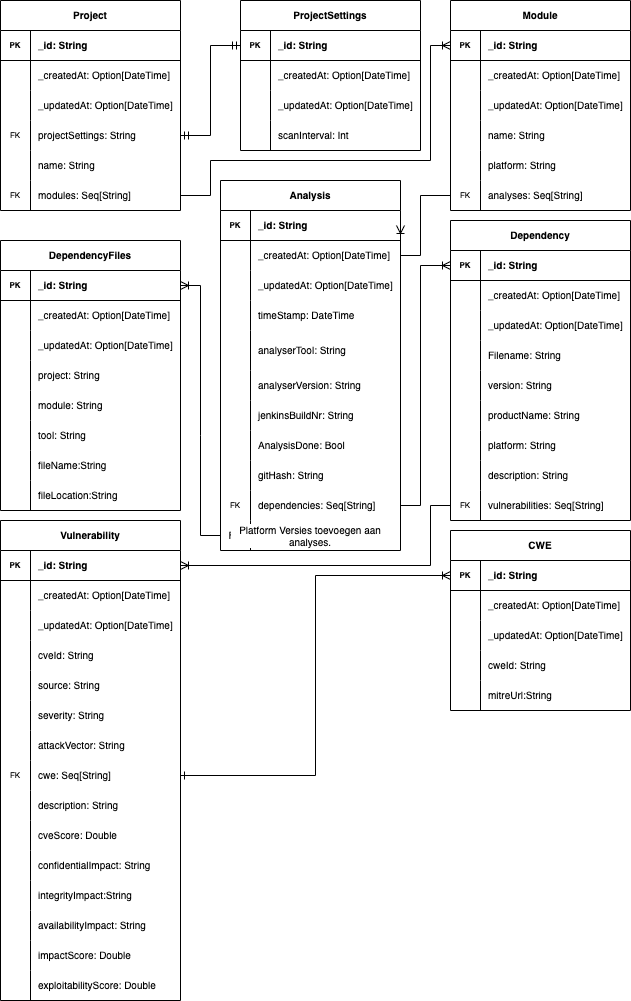
\includegraphics[width=15cm]{gfx/SOUPAPI-SOUPAPI DM}
    \caption{Intern Datamodel}
    \label{fig:SOUP-SoupApiDm [CHECKEN]}
\end{figure}

Hieronder wordt iedere entiteit beschreven met daarin het attribuut, het datatype en de reden voor het opslaan van deze data, waarbij geldt dat voor iedere entititeit de volgende attributen standaard zijn \_id, \_createdAt en \_updatedAt opgeslagen.

\begin{tabular}{lll}
    \textbf{Attribuut} & \textbf{Datatype} & \textbf{Notitie}\\
    \_id & String & unique primary key\\
    \_createdAt & DateTime & timestamp aanmaken van record\\
    \_updatedAt & DateTime & timestampt wijzigen van record\\

\end{tabular}
%TODO dit is leidend datamodel bijwerken.
\subsubsection{Project}\label{subsubsec:project}
In deze entititeit worden de basisgegevens van de projecten opgeslagen als ook de relaties met de voor ieder project aanwezige modulen.

\begin{tabular}{lll}
    \textbf{Attribuut} & \textbf{Datatype} & \textbf{Notitie}\\
    projectSettings & String & referentie naar projectsettings\\
    name & String & naam van het project\\
    modules & Seq[String] & bij project horende modules\\

\end{tabular}
\subsubsection{Projectsettings}\label{subsubsec:projectsettings}
Deze enititeit geeft de mogelijkheid tot het opslaan van project specifieke instellingen met betrekking tot de SOUP API\@.

\begin{tabular}{lll}
    \textbf{Attribuut} & \textbf{Datatype} & \textbf{Notitie}\\
    scaninterval  & String & aantal dagen tussen analyses\\
\end{tabular}

\subsubsection{Module}\label{subsubsec:module}
De module is een op zichzelf staand onderdeel van de applicatie geisoleerd door een platform en de specifieke functie. Er kunnen meerdere modules in een project zitten.

\begin{tabular}{lll}
    \textbf{Attribuut} & \textbf{Datatype} & \textbf{Notitie}\\
    name  & String & naam van de module\\
    platform  & String & platform waar de module op geschreven is \\
    analyses  & Seq[String] & reverentie naar alle analyses die gedaan zijn op de module\\
\end{tabular}

\subsubsection{Analysis}\label{subsubsec:analysis}
Een analyse herbergt alle bekende informatie over een module op het moment van de analyse. De dependencies die hier opgeslagen zijn zijn de op dat moment aanwezige dependencies in de module waar de analyse op plaats heeft gevonden. De dependecyfiles worden ook opgeslagen om een periodieke analyse mogelijk te maken op de module die op dat moment bestaat.

\begin{tabular}{lll}
    \textbf{Attribuut} & \textbf{Datatype} & \textbf{Notitie}\\
    timeStamp & DateTime & naam van de module\\
    analyserTool & String & naam van de analyser tool\\
    analyserEngine & String & versie van de SCA tool die gebruikt is\\
    jenkinsBuildNr & Int & JenkinsBuildnr tracebility naar Jenkins\\
    gitHash & String & Githash van een analyseerde module Tracability naar Gitlab\\
    dependencies & Seq[String] & reverentie naar alle dependendencies in de module\\
    dependencyFiles & Seq[String] & reverentie naar alle dependencyFiles gedefinieerd in de module\\
\end{tabular}


\subsubsection{Dependency}\label{subsubsec:dependency}
De Dependency geeft informatie over de bewuste dependency weer waarbij er een referentie is naar een potentiele kwetsbaarheid.

\begin{tabular}{lll}
    \textbf{Attribuut} & \textbf{Datatype} & \textbf{Notitie}\\
    fileName & DateTime & naam van de module\\
    version & String & Naam van de analyser tool\\
    productName & String & Versie van de SCA tool die gebruikt is\\
    platform & Int & JenkinsBuildnr tracebility naar Jenkins\\
    description & String & Githash van  eanalyseerde module Tracability naar Gitlab\\
    vulnerabilities & Seq[String] & Reverentie naar alle dependendencies in de module.\\
\end{tabular}

\subsubsection{Vulberability}\label{subsubsec:vulberability}
Vulnerability geeft de informatie weer over een kwetsbaarheid waaronder het id en de ernst van de kwetsbaarheid. Waarbij het attribuut severity een samenvatting is van alle impact attributen.  De scores zijn opgebouwd middel het model dat door het nvd/nist is opgesteld

\begin{tabular}{lll}
    \textbf{Attribuut} & \textbf{Datatype} & \textbf{Notitie}\\

    cveId & String & ID van de kwetsbaarheid\\
    source & String & de bron waar deze kwetsbaarheid is gevonden\\
    severity & String & algemene indicator van de ernst van de kwetsbaarheid \\
    attackVector & String & Op welke manier de kwetsbaarheid te benutten is\\
    description & String & Algemene beschrijving\\
    cveScore & Double & Algehele score van de kwetsbaarheid\\
    confidentialImpact & String & impact op confidentiality\\
    integrityImpact & String & impact op integrity \\
    availabilityImpact & String &  impact op availability  \\
    impactScore & DOuble & score van de impact door NVD  \\
    exploitabilityScore & Double & Score van exploitability door NVD  \\
    CWE & Seq[String]] & referentie naar de CWE \\
\end{tabular}

\subsubsection{CWE}\label{subsubsec:cwe}
De CWE's bevatten een url naar eventueel meer informatie over de kwetsbaarheid

\begin{tabular}{lll}
    \textbf{Attribuut} & \textbf{Datatype} & \textbf{Notitie}\\
    cweID & String & Het ID van CWE die op mitre te vinden is.\\
    mitreURL & String & de url van de pagina op Mitre(gegenereerd)\\
\end{tabular}

\subsubsection{DependencyFiles}\label{subsubsec:dependencyFiles}
Om op een later stadium een periodieke analyse te kunnen doen worden de dependency files opgeslagen.

\begin{tabular}{lll}
    \textbf{Attribuut} & \textbf{Datatype} & \textbf{Notitie}\\
    project & String & Referentie naar Project\\
    module & String & Referentie naar module \\
    fileName & String & filename van het bestand \\
    partnerFile & Seq[String] & Reverentie naar andere benodigde bestanden.\\
    platform & String & gebruikte platform \\
    filePath & String & path naar het opgeslagen bestand \\ %TODO AAngepast
    nodeversion & String & versie van Node  \\
    npmversion & String & versie van NPM  \\
    sbtversion & String & versie van Version  \\
    scalaversion & String & versie van scala  \\
    javaversion & String & versie van java \\
\end{tabular}

\subsection{Portal Datamodel}\label{subsec:portal-datamodel}
Om over de mogelijkheid te beschikken om een samenvatting te verkrijgen over kwetsbaarheden per project en per module moet er in de portal een aantal entiteiten worden toegevoegd. Het ontwerp dat hier getoont is een toevoeging op het bestaande model en wordt niet in zijn geheel getoont, maar enkel de aangegrenzende entiteiten en de aanpassingen hierop.

Voor de functionaliteit van de SOUP module binnen de portal moeten er twee entiteiten worden toegevoegd namelijk $'$Module$'$ voor het weergeven van module data in projecten en $'$VulnerabilitySummary$'$ waarin de de waarden worden opgeslagen die weergegeven worden in de portal. De keuze om deze gegevens toe te voegen in het datamodel van de Portal is performance. Vaak is het alleen van belang om de samenvatting te kunnen lezen en op het moment dat er teveel kwetsbaarheden gevonden worden kan er naar de details in de SOUPAPI worden gekeken. Om deze reden is het niet nodig om alle beschikbare info over te sturen gezien het in het geval van NPM vaak tot honderden dependencies kan leiden.


\begin{figure}[bth]
    \myfloatalign
    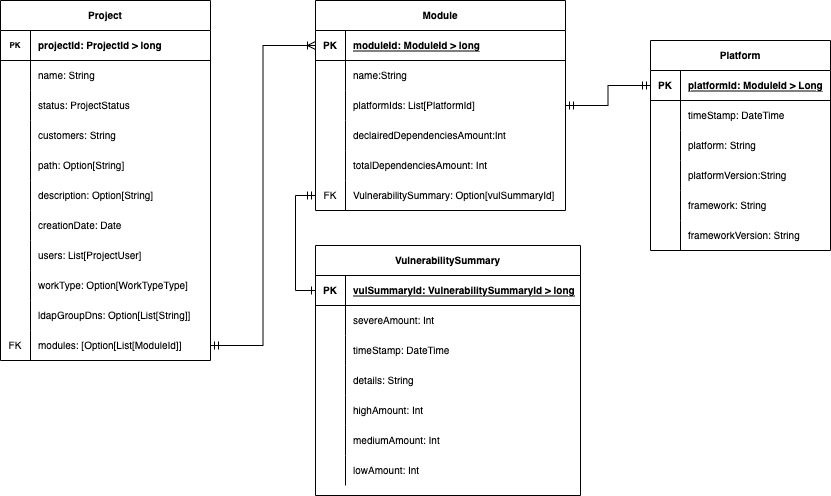
\includegraphics[width=15cm]{gfx/SOUPAPI-PortalDM}
    \caption{Toevoegingen op het bestaande portal Datamodel}
    \label{fig:SOUP-portalDm}
\end{figure}
\clearpage
\subsubsection{Project}\label{subsubsec:portalProject}
Dit is een bestaande entiteit binnen het huidige portal project. Hierin worden de gegevens opgeslagen die te maken hebben met de projecten die binnen Eaglescience bestaan. Dit zijn zowel Draft (nieuwe), active, en archived projecten.

\begin{tabular}{lll}
    \textbf{Attribuut} & \textbf{Datatype} & \textbf{Notitie}\\
    projectId & ProjectId > Long & uniek id\\
    status & ProjectStatus & [enum] status van het project\\
    customers & String & projectklant\\
    path & Option[String] & projectPath\\
    description & Option[String] & beschrijving van het project\\
    creationDate & Date & aanmaakdatum van het project \\
    users & List[ProjectUser] & Eaglescience medewerkers op het project \\
    workType & Option[WorkTypeType] & welk werk is er belegt in het project   \\
    ldapGroupDns & Option[List[String]] & welke group heeft het project in LDAP  \\
    modules & Option[List[String]] & referentie naar de aanwezige modules  \\
\end{tabular}

\subsubsection{Module}\label{subsubsec:portalModule}
De module entiteit slaat de gegevens op voor een specifieke module, met een referentie naar een lijst van samenvattingen.

\begin{tabular}{lll}
    \textbf{Attribuut} & \textbf{Datatype} & \textbf{Notitie}\\
    moduleId & ModuleId > Long & uniek id \\
    name & String & referentie naar Project\\
    platform & String & gebruikte platform \\
    platformversion & String & versie van Node  \\
    framework & String &  gebruikte framework  \\
    frameworkVersion & String & versie van framework  \\
    declairedDepAmnt & Int & aantal opgegeven dependencies\\
    totaalDepAmnt & Int & totaal aantal dependencies\\
    vulSummaries & Option[List[VulSumId]]& referentie naar samenvatting\\
\end{tabular}

\subsubsection{Vulnerability Summary}\label{subsubsec:portalVulSum}
Ieder moment dat er een analyse is uitgevoerd wordt er hier een samenvating aan toegevoegd, zodat er een up to date samenvatting beschikbaar is voor de portal evenals de geschiedenis hiervan.

\begin{tabular}{lll}
    \textbf{Attribuut} & \textbf{Datatype} & \textbf{Notitie}\\
    vulSummaryId & VulSumId > Long & uniek Id\\
    timeStamp & DataTime & moment van opslaan van de samenvating\\
    details & String & referentie naar SOUPAPI model analyse\\
    severeAmount & Int & aantal Severe kwetsbaarheden\\
    highAmount & Int & aantal High kwetsbaarheden\\
    mediumAmount & Int & aantal Medium kwetsbaarheden\\
    lowAmount & Int & aantal Low kwetsbaarheden\\
\end{tabular}

\section{Algemene Architectuur}\label{sec:algemene-architectuur}
%TODO tekst beter structureren

Voor het analyseren, beheren en weergeven van een SOUP-analyse heeft de applicatie een aantal componenten nodig die elk een eigen verantwoordelijkheid hebben in de taken die de applicatie uit moet voeren. Om deze verantwoordelijkheden te splitsen is de applicatie opgesplitst in verschillende modulen. Voor sommige onderdelen geldt zelfs dat het zelf een onderdeel is van een andere applicatie binnen de Eaglescience Dev-stack. Voor een volledige compatibiliteit wordt de applicatie in Scala geschreven waarbij het PlayFramework wordt gebruikt. Voor Frontend delen en dan met name in de portal wordt er Angular gebruikt, omdat dit hier al gebruikt wordt. Zoals te zien is in figuur~\ref{fig:SOUP-Components} zijn er verschillende componenten die samen werken om een analyse weer te geven voor de gebruiker.

\textbf{Jenkins} is verantwoordelijk voor het up-to-date houden van de laatste wijzigingen in de sourde-code en het initiele rapport, welke aangeboden wordt aan de \textbf{SOUP-API}. Hierin is de  \textbf{ReportParserEngine} verantwoordelijk voor het omzetten van de binnegekomen rapporten naar het interne datamodel. De \textbf{PeriodicAnalysisEngine} is verantwoordelijk voor het doen van periodieke analyses met de dependency declaraties. Centraal in de SOUP-API staat de \textbf{API} welke verantwoordelijk is voor de dataverwerking van de data die door de beide engines gegenereerd of benodigd is. Daarnaast is het verantwoordelijk voor het opslaan van de dependency declaraties. De \textbf{Portal} is verantwoordelijk voor de user interface met de gebruiker en de SOUP-API. Voor periodieke analyse van de modules binnen projecten is er een \textbf{AnalysisEnvironment} welke zorg draagt voor de veilige analyse van modules op basis van de laatst opgeslagen dependencyDeclaraties. Als \textbf{Database} is MongoDB gekozen omdat er wisselingen in content kan zitten van de uitslagen en dit een flexibelere manier van opslaan vereist is.
In de komende secties zal er dieper ingegaan worden op de verschillende componten waardoor er een completer beeld hierover onstaat. Functionele ontwerpen zullen worden aangeboden in de hierop volgende hoofdstukken.

\begin{figure}[bth]
    \myfloatalign
    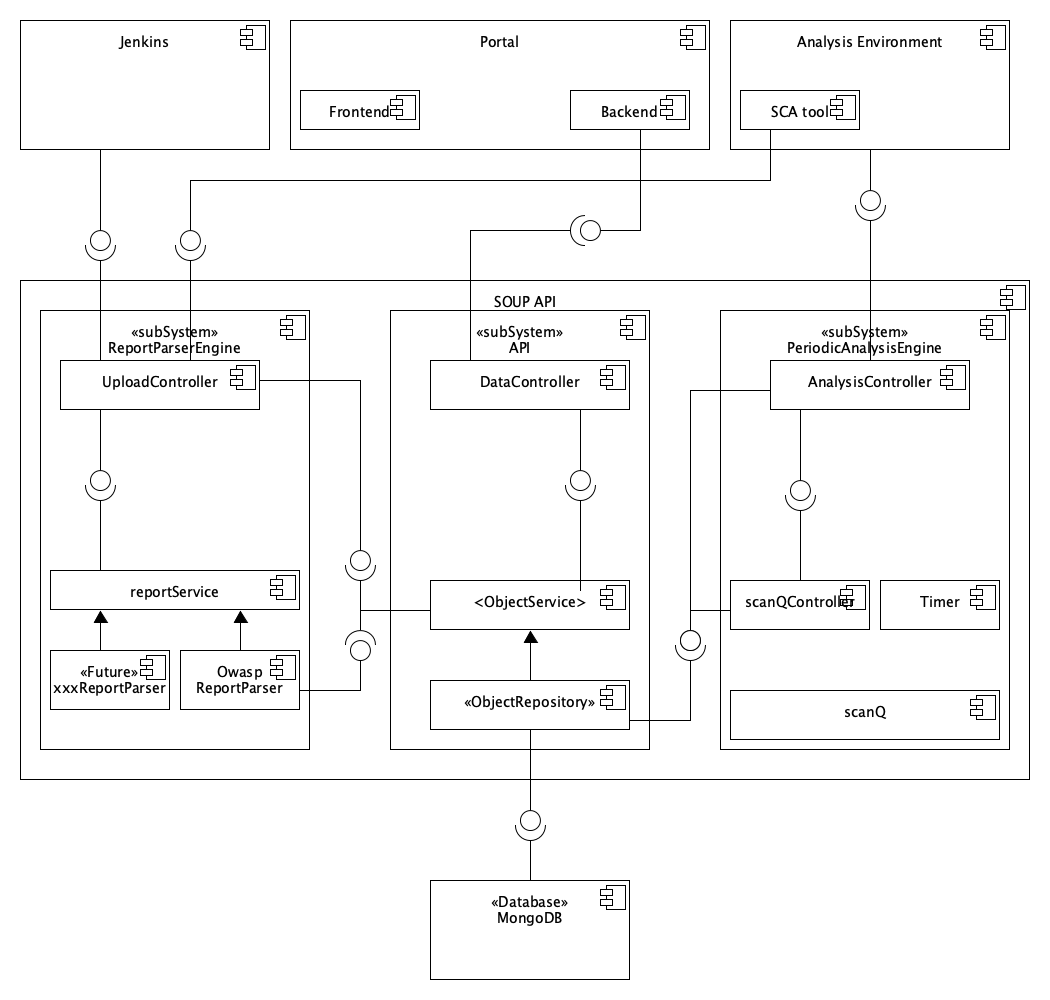
\includegraphics[width=17cm]{gfx/umlet/exports/ApplicationComponents}
    \caption{Componenten SOUP Analyse Systeem}
    \label{fig:SOUP-Components}
\end{figure}
\clearpage
\section{SOUP API}\label{sec:soup-api}
De SOUP-API is een opzichzelf staand centraal deel van de applicatie welke verantwoordelijk is voor de verwerking van gegevens uit de SCA tooling en de portal. Hiernaast regelt het ook de periodieke analyses om informatie up-to-date te houden van al eerder geanalyseerde projecten waar al een tijd geen wijzigingen op zijn geweest. Deze verantwoordelijkheden worden door de volgende componenten beheert:

\subsection{ReportParseEngine}\label{subsec:reportparseengine}
De ReportParseEngine zorgt ervoor dat de binnenkomende datastroom vanuit de SCA tooling wordt verwerkt tot gegevens die in de SOAP-API gebruikt kan worden om inzichten in kwetsbaarheden te verkrijgen.

\begin{figure}[bth]
    \myfloatalign
    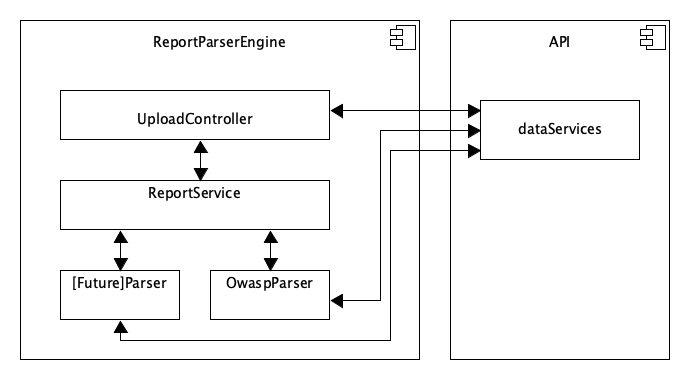
\includegraphics[width=8cm]{gfx/umlet/exports/ReportParserComponents}
    \caption{Componenten SOUP-API ReportParser}
    \label{fig:SOUPAPIReportParserComps}
\end{figure}

De datastroom die binnen komt bestaat uit een aantal zaken. Ten eerste is er het rapport dat uit de SCA tooling komt dat omgezet moet worden naar het intene datamodel. Ten tweede zal er metadata worden verstuurt die de API gebruikt om de analyses op de juiste plek op te slaan. Om de verantwoordelijkheden goed te verdelen zijn er een aantal services voorzien:

De \textbf{ParserService} is het centrale aanspreek punt van de ReportParseEngine en heeft als taak dat de juiste functionaliteit wordt aangesproken op het moment dat bepaalde vormen van instroom data worden aangeboden. De ReportParseEngine moet de mogelijkheid hebben om in de toekomst met meer SCA tools om te kunnen gaan. De verwachting is dat niet iedere tool dezelfde opmaak van het rapport heeft en er om die redenen meerdere parsers moeten worden ontwikkeld in figuur~\ref{fig:SOUPAPIReportParserComps} staat deze aangegeven als $"$FutureParser$"$.

De \textbf{OWASP Parser} maakt het mogelijk om het rapport dat gegenereerd wordt door de OWASP tool \footnote{tooling die is voortgekomen uit het hiervoor beschreven onderzoek} om te zetten naar data in de database. Naast het plaatsen van de data in de interne database genereert het ook een samenvatting die in database van de portal wordt geplaatst.

\subsection{Periodic Analysis Engine}\label{subsec:periodicanalysisengine}
De Periodic Analysis Engine is een module die verantwoordelijk is voor het periodiek analyseren van modulen. Een schematische weergave is te zien in figuur~\ref{fig:SOUPAPIPeriodicAnalysisEngineComps}. Deze modulen worden in een lijst genaamd de \textbf{scanQ} opgeslagen welke door de \textbf{scanQservice} wordt beheerd. Deze service is verantwoordelijk voor alle mutaties op de lijst als ook voor het ophalen van data welke bekend is voor de module. Op die manier krijgt de Analyses Environment de juiste gegevens om een container op te kunnen zetten. De algehele controle wordt uitgevoerd door de \textbf{AnalysisController} welke verantwoordelijk is voor het starten van de gewenste analyse.

\begin{figure}[bth]
    \myfloatalign
    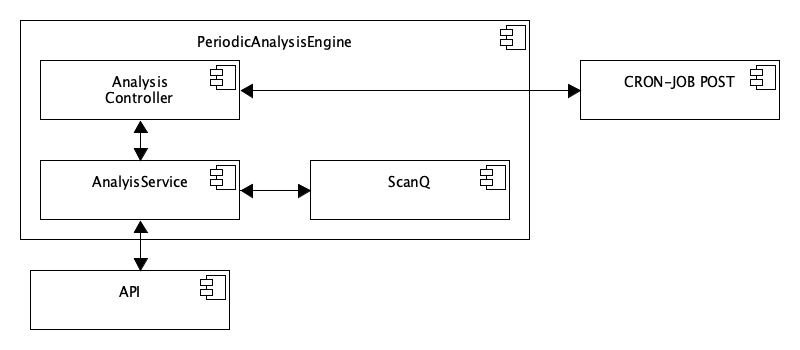
\includegraphics[width=8cm]{gfx/umlet/exports/PeriodicAnalyisEngineComponents}
    \caption{Componenten SOUP-API Periodic Analysis Engine}
    \label{fig:SOUPAPIPeriodicAnalysisEngineComps}
\end{figure}

\newpage %TODO: Tijdelijk voor placering van de afbeeldingen later testen of zonder ook goed uitziet.
\subsection{API}\label{subsec:api2}
De voornaamste verantwoordelijkheid van de API is ervoor zorgdragen dat de data die in de SOUP-API wordt gemuteerd in de interne database wordt opgeslagen, en daarnaast deze data beschikbaar te stellen voor services en modulen die hier afhankelijk van zijn. Zie figuur ~\ref{fig:SOUPAPI-API comps}. De API is opgebouwd volgens een Controller, Service, Repository architectuur waarbij de Controller verantwoordelijk is voor het beschikbaar stellen van services op verschillende REST-endpoints. De Service zelf is verantwoordelijk voor de business logica en mutatie van de data, welke vervolgens door de Repository wordt weggeschreven naar de database.
\begin{figure}[bth]
    \myfloatalign
    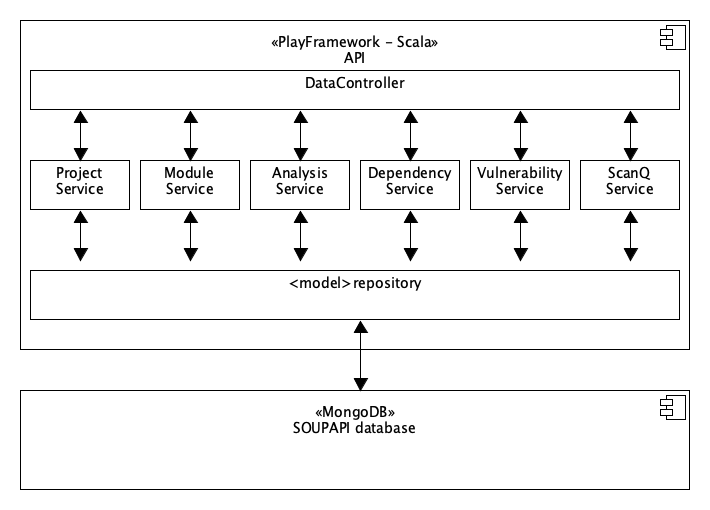
\includegraphics[width=15cm]{gfx/umlet/exports/API-ComponentsDiagram}
    \caption{Componenten API binnen de SOUP-API}
    \label{fig:SOUPAPI-API comps}
\end{figure}

Naast services en een datacontroller die verantwoordelijk is voor de mutatie van alle data, is er ook een UploadController die samen met een reportService verantwoordelijk is voor het aansturen van de ReportParseEngine. De reportService verwerkt ook de dependencyFiles die vanuit Jenkins worden verstuurt.

\section{Software Compsition Analysis in Jenkins}\label{sec:jenkins}
De bestaande Jenkins omgeving is de primaire bron voor nieuwe informatie uit projecten. Het aangewezen moment in de ontwikkelingsCyclus voor het uitvoeren van een analyses is wanneer er een acceptatie of productie build wordt uitgevoerd. De eerste reden hiervoor is omdat op dit moment de dependencies relatief vast staan ten opzichte van eerdere fasen in de ontwikkeling. De tweede reden is dat de development/ personal builds veel frequenter voorkomen en dat de performance van deze builds door de hieronder besproken toevoegingen achteruit kan gaan. In figuur ~\ref{fig:JenkinsSequece} is deze sequentie weergegeven.


\begin{figure}[bth]
    \myfloatalign
    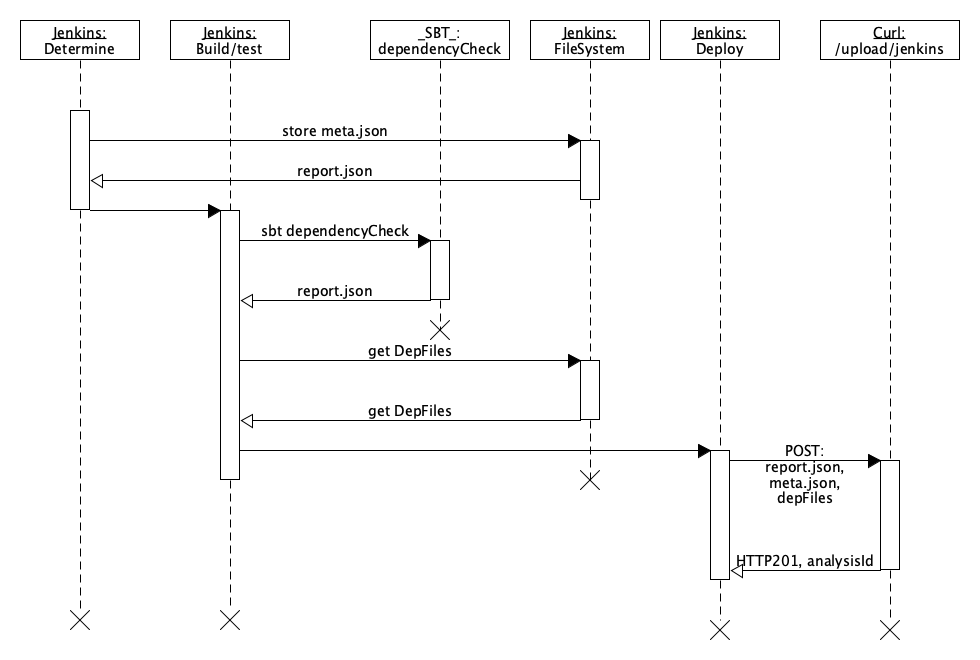
\includegraphics[width=15cm]{gfx/umlet/exports/jenkinsBuildSequence}
    \caption{Jenkins Buildsequence: alleen onderdelen relavant voor SOUP-API worden getoont}
    \label{fig:JenkinsSequece}
\end{figure}

De pipeline binnen Jenkins kent voor de SOUP-API twee belangrijke momenten. In de \textbf{build/test fase} waarin de module wordt gebouwd en vervolgens getest zullen er twee toevoegingen gedaan moeten worden. Als eerst moet er meta data worden gepubliceerd op het filesysteem zodat er in een later stadium bekend is welke module, jenkins buildnummer en githash geanalyseerd wordt. Dit waarborgt de traceability tussen Jenkins, gitlab en de SOUPAPI. Later moet in die zelfde stap de SCA tool worden uitgevoerd om de module te analyseren op kwetsbaarheden. Het resultaat van deze analyse wordt vervolgens gepubliceerd op het filesysteem.

Op het moment dat de \textbf{deploy} fase gelukt is kan er een upload plaatsvinden naar de SOUP API met daarin: "report.json, meta.json" en dependency declaraties als (build.sbt/dependencies.scala of de package-lock.json)
Als de upload lukt dan zal Jenkins de build vrijgeven als geslaagd. Mocht er onverhoopt iets niet lukken in de upload zal dit te zien zijn in de logs van Jenkins.

\section{Portal}\label{sec:arch-portal} De portal is een inhouse applicatie welke gebruikt wordt voor administratieve zaken binnen het bedrijf. De wens is om hier functionaliteiten aan toe te voegen die bedrijfsbreed zijn en daarmee dus project oversteigend. Voor deze applicatie dient er een module te worden toeegevoegd die fungeert als een interface waarin informatie over de bekende kwetsbaarheden te vinden is, maar ook instellingen omtrend de SOUP-API kunnen worden aangepast. Er bestaat nu een module dat projects heet waarin verschillende details van het project in opgeslagen worden. Samenvatingen van informatie over kwetsbaarheden kunnen hieraan worden toegevoegd.
Daarnaast zal er een nieuwe module moeten worden ontwikkeld waarin de details van de analyses kunnen worden gevonden. Deze module moet samenwerken met de SOUP-API API om de gewenste gegevens te kunnen weergeven.

\section{Analysis Environment}\label{sec:analysis-environment}
Deze omgeving moet het mogelijk maken om vanuit de SOUP-API een analyse uit te voeren op modulen, waarbij er eerst een docker container wordt gestart, hier vervolgens een analyse in wordt uitgevoerd en gepubliceers waarna de container wordt vernietigd. De voornaamste reden voor het uitvoeren van analyses op deze manier is dat er hierdoor de analyse container exact dezelfde runtime versies heeft als die op de productie. Naast de grote variatie in omgevingen is er ook de mogelijkheid dat er ergens in een declaratie van dependencies code staat die uitgevoerd kan worden middels install scripts. Om ervoor te zorgen dat deze geen blijvend effect hebben op het systeem wordt er gekozen voor een docker systeem wat iedere keer opnieuw kan worden geinitialiseerd.

\section{Deployment}\label{sec:deployment}


\begin{figure}[bth]
    \myfloatalign
    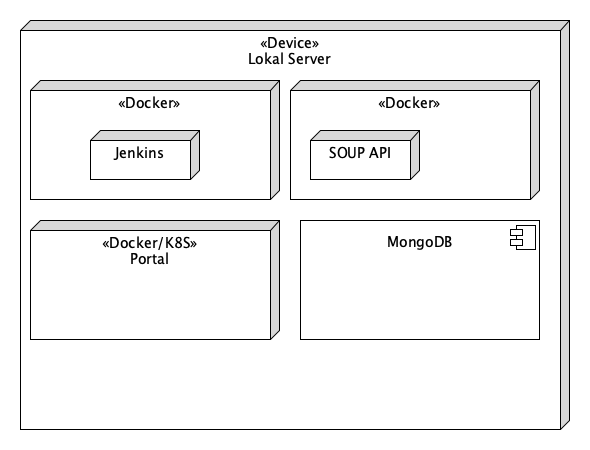
\includegraphics[width=10cm]{gfx/umlet/exports/deployment}
    \caption{Deployment }
    \label{fig:deployment}
\end{figure}

De portal draait lokaal binnen Eaglscience in een docker omgeving. De frontend is geschreven in Angular 13, waarbij er tegen een backend wordt gecommuniceerd welke in Scala 2.13 is geschreven met PlayFramework. De SOUP-API is een opzichzelfstaand component binnen de gehele applicatie en zal ook worden geschreven in Scala met PlayFramework. De SOUP-API zal worden ondergebracht in een dockercontainer welk beschikbaar is voor de portal, Jenkins en de database. De database is een mongoDB database en zal ook moeten worden ingericht. Het maakt voor de werking niet veel uit of dit een lokale database of een instantie in de cloud is.

\subsection{Gebruikte platformen en systemen NIEUW}
De SOUP-API wordt gescheven in Scala met als webframework PlayFramework, een framework dat het ontwikkelen van webapplicaties ondersteunt. Om met MongoDB te kunnen communiceren is de bibliotheek ReactiveMongo gekozen om ervoor te zorgen dat de reactive aard van Play niet wordt onderbroken door Database bewerkingen. De SOUP-API gaat in een eigen docker container draaien om op die manier makkelijk te kunnen deployen. De portal is al geschreven in angular 13 en de module die toegevoegd zal worden zal hierin meegaan.
De Analyse omgeving waar de periodieke analyses op kwetsbaarheden plaats gaat vinden zal ook  een docker omgeving zijn. De voornaamste reden is dat door de vluchtige aard van containers de omgevingen makkelijk kunnen worden opgezet, de analyse gedaan kan worden en vervolgens weer kan worden vernietigd.

